\documentclass[twoside]{book}

% Packages required by doxygen
\usepackage{fixltx2e}
\usepackage{calc}
\usepackage{doxygen}
\usepackage[export]{adjustbox} % also loads graphicx
\usepackage{graphicx}
\usepackage[utf8]{inputenc}
\usepackage{makeidx}
\usepackage{multicol}
\usepackage{multirow}
\PassOptionsToPackage{warn}{textcomp}
\usepackage{textcomp}
\usepackage[nointegrals]{wasysym}
\usepackage[table]{xcolor}

% Font selection
\usepackage[T1]{fontenc}
\usepackage[scaled=.90]{helvet}
\usepackage{courier}
\usepackage{amssymb}
\usepackage{sectsty}
\renewcommand{\familydefault}{\sfdefault}
\allsectionsfont{%
  \fontseries{bc}\selectfont%
  \color{darkgray}%
}
\renewcommand{\DoxyLabelFont}{%
  \fontseries{bc}\selectfont%
  \color{darkgray}%
}
\newcommand{\+}{\discretionary{\mbox{\scriptsize$\hookleftarrow$}}{}{}}

% Page & text layout
\usepackage{geometry}
\geometry{%
  a4paper,%
  top=2.5cm,%
  bottom=2.5cm,%
  left=2.5cm,%
  right=2.5cm%
}
\tolerance=750
\hfuzz=15pt
\hbadness=750
\setlength{\emergencystretch}{15pt}
\setlength{\parindent}{0cm}
\setlength{\parskip}{3ex plus 2ex minus 2ex}
\makeatletter
\renewcommand{\paragraph}{%
  \@startsection{paragraph}{4}{0ex}{-1.0ex}{1.0ex}{%
    \normalfont\normalsize\bfseries\SS@parafont%
  }%
}
\renewcommand{\subparagraph}{%
  \@startsection{subparagraph}{5}{0ex}{-1.0ex}{1.0ex}{%
    \normalfont\normalsize\bfseries\SS@subparafont%
  }%
}
\makeatother

% Headers & footers
\usepackage{fancyhdr}
\pagestyle{fancyplain}
\fancyhead[LE]{\fancyplain{}{\bfseries\thepage}}
\fancyhead[CE]{\fancyplain{}{}}
\fancyhead[RE]{\fancyplain{}{\bfseries\leftmark}}
\fancyhead[LO]{\fancyplain{}{\bfseries\rightmark}}
\fancyhead[CO]{\fancyplain{}{}}
\fancyhead[RO]{\fancyplain{}{\bfseries\thepage}}
\fancyfoot[LE]{\fancyplain{}{}}
\fancyfoot[CE]{\fancyplain{}{}}
\fancyfoot[RE]{\fancyplain{}{\bfseries\scriptsize Generated by Doxygen }}
\fancyfoot[LO]{\fancyplain{}{\bfseries\scriptsize Generated by Doxygen }}
\fancyfoot[CO]{\fancyplain{}{}}
\fancyfoot[RO]{\fancyplain{}{}}
\renewcommand{\footrulewidth}{0.4pt}
\renewcommand{\chaptermark}[1]{%
  \markboth{#1}{}%
}
\renewcommand{\sectionmark}[1]{%
  \markright{\thesection\ #1}%
}

% Indices & bibliography
\usepackage{natbib}
\usepackage[titles]{tocloft}
\setcounter{tocdepth}{3}
\setcounter{secnumdepth}{5}
\makeindex

% Hyperlinks (required, but should be loaded last)
\usepackage{ifpdf}
\ifpdf
  \usepackage[pdftex,pagebackref=true]{hyperref}
\else
  \usepackage[ps2pdf,pagebackref=true]{hyperref}
\fi
\hypersetup{%
  colorlinks=true,%
  linkcolor=blue,%
  citecolor=blue,%
  unicode%
}

% Custom commands
\newcommand{\clearemptydoublepage}{%
  \newpage{\pagestyle{empty}\cleardoublepage}%
}

\usepackage{caption}
\captionsetup{labelsep=space,justification=centering,font={bf},singlelinecheck=off,skip=4pt,position=top}

%===== C O N T E N T S =====

\begin{document}

% Titlepage & ToC
\hypersetup{pageanchor=false,
             bookmarksnumbered=true,
             pdfencoding=unicode
            }
\pagenumbering{roman}
\begin{titlepage}
\vspace*{7cm}
\begin{center}%
{\Large My Project }\\
\vspace*{1cm}
{\large Generated by Doxygen 1.8.11}\\
\end{center}
\end{titlepage}
\clearemptydoublepage
\tableofcontents
\clearemptydoublepage
\pagenumbering{arabic}
\hypersetup{pageanchor=true}

%--- Begin generated contents ---
\chapter{Hierarchical Index}
\section{Class Hierarchy}
This inheritance list is sorted roughly, but not completely, alphabetically\+:\begin{DoxyCompactList}
\item \contentsline{section}{adc}{\pageref{classadc}}{}
\item Task\+Base\begin{DoxyCompactList}
\item \contentsline{section}{task\+\_\+brightness}{\pageref{classtask__brightness}}{}
\item \contentsline{section}{task\+\_\+user}{\pageref{classtask__user}}{}
\end{DoxyCompactList}
\end{DoxyCompactList}

\chapter{Class Index}
\section{Class List}
Here are the classes, structs, unions and interfaces with brief descriptions\+:\begin{DoxyCompactList}
\item\contentsline{section}{\hyperlink{classadc}{adc} \\*This class runs the A/D converter on an A\+VR processor }{\pageref{classadc}}{}
\item\contentsline{section}{\hyperlink{classtask__brightness}{task\+\_\+brightness} \\*This task controls the brightness of an L\+ED using an analog input from the A/D converter }{\pageref{classtask__brightness}}{}
\item\contentsline{section}{\hyperlink{classtask__user}{task\+\_\+user} }{\pageref{classtask__user}}{}
\end{DoxyCompactList}

\chapter{File Index}
\section{File List}
Here is a list of all documented files with brief descriptions\+:\begin{DoxyCompactList}
\item\contentsline{section}{\hyperlink{adc_8cpp}{adc.\+cpp} }{\pageref{adc_8cpp}}{}
\item\contentsline{section}{\hyperlink{adc_8h}{adc.\+h} }{\pageref{adc_8h}}{}
\item\contentsline{section}{\hyperlink{main_8cpp}{main.\+cpp} }{\pageref{main_8cpp}}{}
\item\contentsline{section}{\hyperlink{shares_8h}{shares.\+h} }{\pageref{shares_8h}}{}
\item\contentsline{section}{\hyperlink{task__brightness_8cpp}{task\+\_\+brightness.\+cpp} }{\pageref{task__brightness_8cpp}}{}
\item\contentsline{section}{\hyperlink{task__brightness_8h}{task\+\_\+brightness.\+h} }{\pageref{task__brightness_8h}}{}
\item\contentsline{section}{\hyperlink{task__user_8cpp}{task\+\_\+user.\+cpp} }{\pageref{task__user_8cpp}}{}
\item\contentsline{section}{\hyperlink{task__user_8h}{task\+\_\+user.\+h} }{\pageref{task__user_8h}}{}
\end{DoxyCompactList}

\chapter{Class Documentation}
\hypertarget{classadc}{}\section{adc Class Reference}
\label{classadc}\index{adc@{adc}}


This class runs the A/D converter on an A\+VR processor.  




{\ttfamily \#include $<$adc.\+h$>$}

\subsection*{Public Member Functions}
\begin{DoxyCompactItemize}
\item 
\hyperlink{classadc_af3b8262c08f5fc5ae325a20622883424}{adc} (emstream $\ast$=N\+U\+LL)
\begin{DoxyCompactList}\small\item\em This constructor sets up an A/D converter. \end{DoxyCompactList}\item 
uint16\+\_\+t \hyperlink{classadc_a2190a59696a7093e1ea605e998ccf97e}{read\+\_\+once} (uint8\+\_\+t)
\begin{DoxyCompactList}\small\item\em This method takes one A/D reading from the given channel and returns it. \end{DoxyCompactList}\item 
uint16\+\_\+t \hyperlink{classadc_a58f1030fe64d3dea4ccd8a2687dd6fce}{read\+\_\+oversampled} (uint8\+\_\+t, uint8\+\_\+t)
\begin{DoxyCompactList}\small\item\em This takes an averaged A/D reading from a given number of samples. \end{DoxyCompactList}\end{DoxyCompactItemize}
\subsection*{Protected Attributes}
\begin{DoxyCompactItemize}
\item 
emstream $\ast$ \hyperlink{classadc_a14680b48b723bf1adddd2741ebb18a3e}{ptr\+\_\+to\+\_\+serial}\hypertarget{classadc_a14680b48b723bf1adddd2741ebb18a3e}{}\label{classadc_a14680b48b723bf1adddd2741ebb18a3e}

\begin{DoxyCompactList}\small\item\em The A\+DC class uses this pointer to the serial port to dump all the A/D inputs to the serial for debugging purposes. \end{DoxyCompactList}\end{DoxyCompactItemize}


\subsection{Detailed Description}
This class runs the A/D converter on an A\+VR processor. 

These are some simple drivers to handle analog readings on the ME 405 board. 

\subsection{Constructor \& Destructor Documentation}
\index{adc@{adc}!adc@{adc}}
\index{adc@{adc}!adc@{adc}}
\subsubsection[{\texorpdfstring{adc(emstream $\ast$=\+N\+U\+L\+L)}{adc(emstream *=NULL)}}]{\setlength{\rightskip}{0pt plus 5cm}adc\+::adc (
\begin{DoxyParamCaption}
\item[{emstream $\ast$}]{p\+\_\+serial\+\_\+port = {\ttfamily NULL}}
\end{DoxyParamCaption}
)}\hypertarget{classadc_af3b8262c08f5fc5ae325a20622883424}{}\label{classadc_af3b8262c08f5fc5ae325a20622883424}


This constructor sets up an A/D converter. 

The A/D is made ready so that when a method such as {\ttfamily \hyperlink{classadc_a2190a59696a7093e1ea605e998ccf97e}{read\+\_\+once()}} is called, correct A/D conversions can be performed. T\+O\+DO\+: This code is supplied as gibberish which isn\textquotesingle{}t very usable for much besides verifying that the A/D can work. It should be re-\/written in a useful and readable way, and this comment should be changed to {\bfseries say} {\bfseries something} {\bfseries useful}. 
\begin{DoxyParams}{Parameters}
{\em p\+\_\+serial\+\_\+port} & A pointer to the serial port which writes debugging info. \\
\hline
\end{DoxyParams}


\subsection{Member Function Documentation}
\index{adc@{adc}!read\+\_\+once@{read\+\_\+once}}
\index{read\+\_\+once@{read\+\_\+once}!adc@{adc}}
\subsubsection[{\texorpdfstring{read\+\_\+once(uint8\+\_\+t)}{read_once(uint8_t)}}]{\setlength{\rightskip}{0pt plus 5cm}uint16\+\_\+t adc\+::read\+\_\+once (
\begin{DoxyParamCaption}
\item[{uint8\+\_\+t}]{ch}
\end{DoxyParamCaption}
)}\hypertarget{classadc_a2190a59696a7093e1ea605e998ccf97e}{}\label{classadc_a2190a59696a7093e1ea605e998ccf97e}


This method takes one A/D reading from the given channel and returns it. 

This code clears the M\+UX Selection first, and turns off some features we don\textquotesingle{}t use at first. T\+O\+DO\+: This code is supplied as gibberish which isn\textquotesingle{}t very usable for much besides verifying that the A/D can work. It should be re-\/written in readable C++. Also, the case of a timeout should be gracefully handled; the current minimal mess can hang in certain circumstances. And make sure to {\bfseries fix} {\bfseries this} {\bfseries comment!} 
\begin{DoxyParams}{Parameters}
{\em ch} & The A/D channel which is being read must be from 0 to 7 \\
\hline
\end{DoxyParams}
\begin{DoxyReturn}{Returns}
The result of the A/D conversion 
\end{DoxyReturn}
\index{adc@{adc}!read\+\_\+oversampled@{read\+\_\+oversampled}}
\index{read\+\_\+oversampled@{read\+\_\+oversampled}!adc@{adc}}
\subsubsection[{\texorpdfstring{read\+\_\+oversampled(uint8\+\_\+t, uint8\+\_\+t)}{read_oversampled(uint8_t, uint8_t)}}]{\setlength{\rightskip}{0pt plus 5cm}uint16\+\_\+t adc\+::read\+\_\+oversampled (
\begin{DoxyParamCaption}
\item[{uint8\+\_\+t}]{channel, }
\item[{uint8\+\_\+t}]{samples}
\end{DoxyParamCaption}
)}\hypertarget{classadc_a58f1030fe64d3dea4ccd8a2687dd6fce}{}\label{classadc_a58f1030fe64d3dea4ccd8a2687dd6fce}


This takes an averaged A/D reading from a given number of samples. 

It runs a basic F\+OR loop in code, taking multiple readings and averaging them before returning the average input. 
\begin{DoxyParams}{Parameters}
{\em channel} & Which A/D channel is being read, from 0 to 7 \\
\hline
{\em samples} & How many samples to take from the A/D converter \\
\hline
\end{DoxyParams}
\begin{DoxyReturn}{Returns}
A/D conversion result, will be between 0 and 1024. 
\end{DoxyReturn}


The documentation for this class was generated from the following files\+:\begin{DoxyCompactItemize}
\item 
\hyperlink{adc_8h}{adc.\+h}\item 
\hyperlink{adc_8cpp}{adc.\+cpp}\end{DoxyCompactItemize}

\hypertarget{classtask__brightness}{}\section{task\+\_\+brightness Class Reference}
\label{classtask__brightness}\index{task\+\_\+brightness@{task\+\_\+brightness}}


This task controls the brightness of an L\+ED using an analog input from the A/D converter.  




{\ttfamily \#include $<$task\+\_\+brightness.\+h$>$}

Inheritance diagram for task\+\_\+brightness\+:\begin{figure}[H]
\begin{center}
\leavevmode
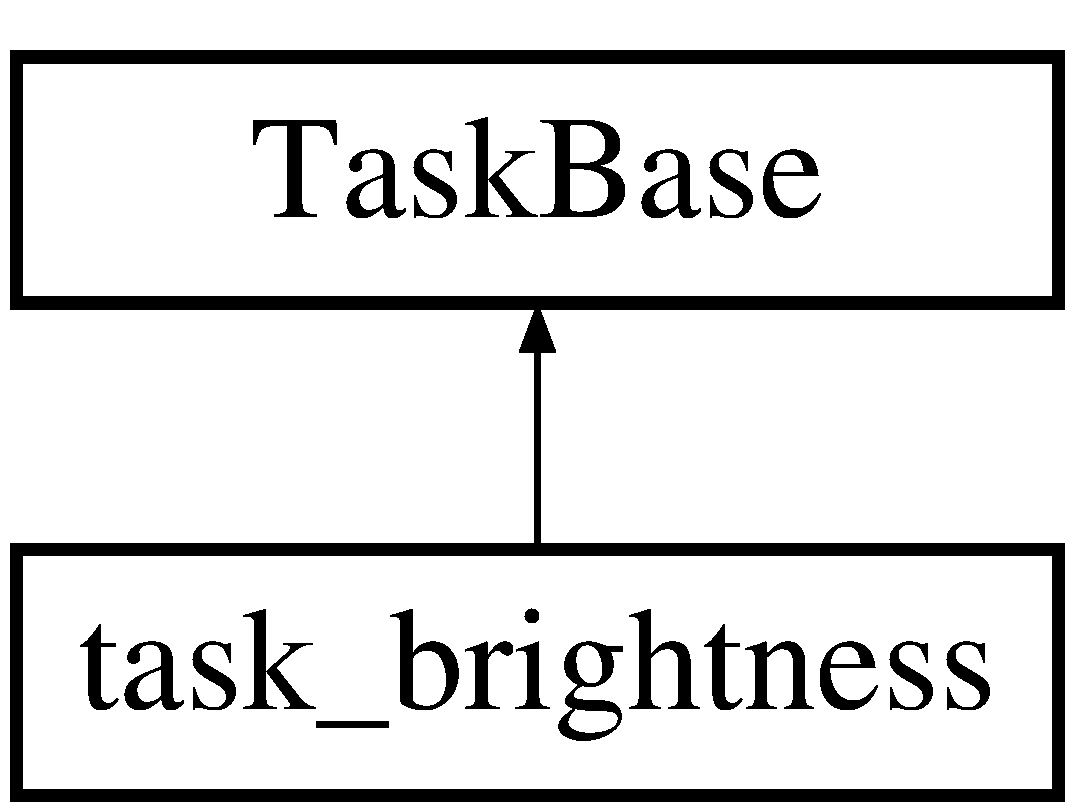
\includegraphics[height=2.000000cm]{classtask__brightness}
\end{center}
\end{figure}
\subsection*{Public Member Functions}
\begin{DoxyCompactItemize}
\item 
\hyperlink{classtask__brightness_a5802baf3a0c9fe53ccbce8966d1fad47}{task\+\_\+brightness} (const char $\ast$, unsigned port\+B\+A\+S\+E\+\_\+\+T\+Y\+PE, size\+\_\+t, emstream $\ast$)
\item 
void \hyperlink{classtask__brightness_a615beac07a99f0856f048a46fd9a3898}{run} (void)
\end{DoxyCompactItemize}


\subsection{Detailed Description}
This task controls the brightness of an L\+ED using an analog input from the A/D converter. 

The A/D converter is run using a driver in files {\ttfamily \hyperlink{adc_8h}{adc.\+h}} and {\ttfamily \hyperlink{adc_8cpp}{adc.\+cpp}}. Code in this task sets up a timer/counter in P\+WM mode and controls the L\+ED\textquotesingle{}s average brightness. 

\subsection{Constructor \& Destructor Documentation}
\index{task\+\_\+brightness@{task\+\_\+brightness}!task\+\_\+brightness@{task\+\_\+brightness}}
\index{task\+\_\+brightness@{task\+\_\+brightness}!task\+\_\+brightness@{task\+\_\+brightness}}
\subsubsection[{\texorpdfstring{task\+\_\+brightness(const char $\ast$, unsigned port\+B\+A\+S\+E\+\_\+\+T\+Y\+P\+E, size\+\_\+t, emstream $\ast$)}{task_brightness(const char *, unsigned portBASE_TYPE, size_t, emstream *)}}]{\setlength{\rightskip}{0pt plus 5cm}task\+\_\+brightness\+::task\+\_\+brightness (
\begin{DoxyParamCaption}
\item[{const char $\ast$}]{a\+\_\+name, }
\item[{unsigned port\+B\+A\+S\+E\+\_\+\+T\+Y\+PE}]{a\+\_\+priority, }
\item[{size\+\_\+t}]{a\+\_\+stack\+\_\+size, }
\item[{emstream $\ast$}]{p\+\_\+ser\+\_\+dev}
\end{DoxyParamCaption}
)}\hypertarget{classtask__brightness_a5802baf3a0c9fe53ccbce8966d1fad47}{}\label{classtask__brightness_a5802baf3a0c9fe53ccbce8966d1fad47}
This constructor creates a task which controls the brightness of an L\+ED using input from an A/D converter. The main job of this constructor is to call the constructor of parent class ({\ttfamily frt\+\_\+task} ); the parent\textquotesingle{}s constructor the work. 
\begin{DoxyParams}{Parameters}
{\em a\+\_\+name} & A character string which will be the name of this task \\
\hline
{\em a\+\_\+priority} & The priority at which this task will initially run (default\+: 0) \\
\hline
{\em a\+\_\+stack\+\_\+size} & The size of this task\textquotesingle{}s stack in bytes (default\+: config\+M\+I\+N\+I\+M\+A\+L\+\_\+\+S\+T\+A\+C\+K\+\_\+\+S\+I\+ZE) \\
\hline
{\em p\+\_\+ser\+\_\+dev} & Pointer to a serial device (port, radio, SD card, etc.) which can be used by this task to communicate (default\+: N\+U\+LL) \\
\hline
\end{DoxyParams}


\subsection{Member Function Documentation}
\index{task\+\_\+brightness@{task\+\_\+brightness}!run@{run}}
\index{run@{run}!task\+\_\+brightness@{task\+\_\+brightness}}
\subsubsection[{\texorpdfstring{run(void)}{run(void)}}]{\setlength{\rightskip}{0pt plus 5cm}void task\+\_\+brightness\+::run (
\begin{DoxyParamCaption}
\item[{void}]{}
\end{DoxyParamCaption}
)}\hypertarget{classtask__brightness_a615beac07a99f0856f048a46fd9a3898}{}\label{classtask__brightness_a615beac07a99f0856f048a46fd9a3898}
This method is called once by the R\+T\+OS scheduler. Each time around the for (;;) loop, it reads the A/D converter and uses the result to control the brightness of an L\+ED. 

The documentation for this class was generated from the following files\+:\begin{DoxyCompactItemize}
\item 
\hyperlink{task__brightness_8h}{task\+\_\+brightness.\+h}\item 
\hyperlink{task__brightness_8cpp}{task\+\_\+brightness.\+cpp}\end{DoxyCompactItemize}

\hypertarget{classtask__user}{}\section{task\+\_\+user Class Reference}
\label{classtask__user}\index{task\+\_\+user@{task\+\_\+user}}


{\ttfamily \#include $<$task\+\_\+user.\+h$>$}

Inheritance diagram for task\+\_\+user\+:\begin{figure}[H]
\begin{center}
\leavevmode
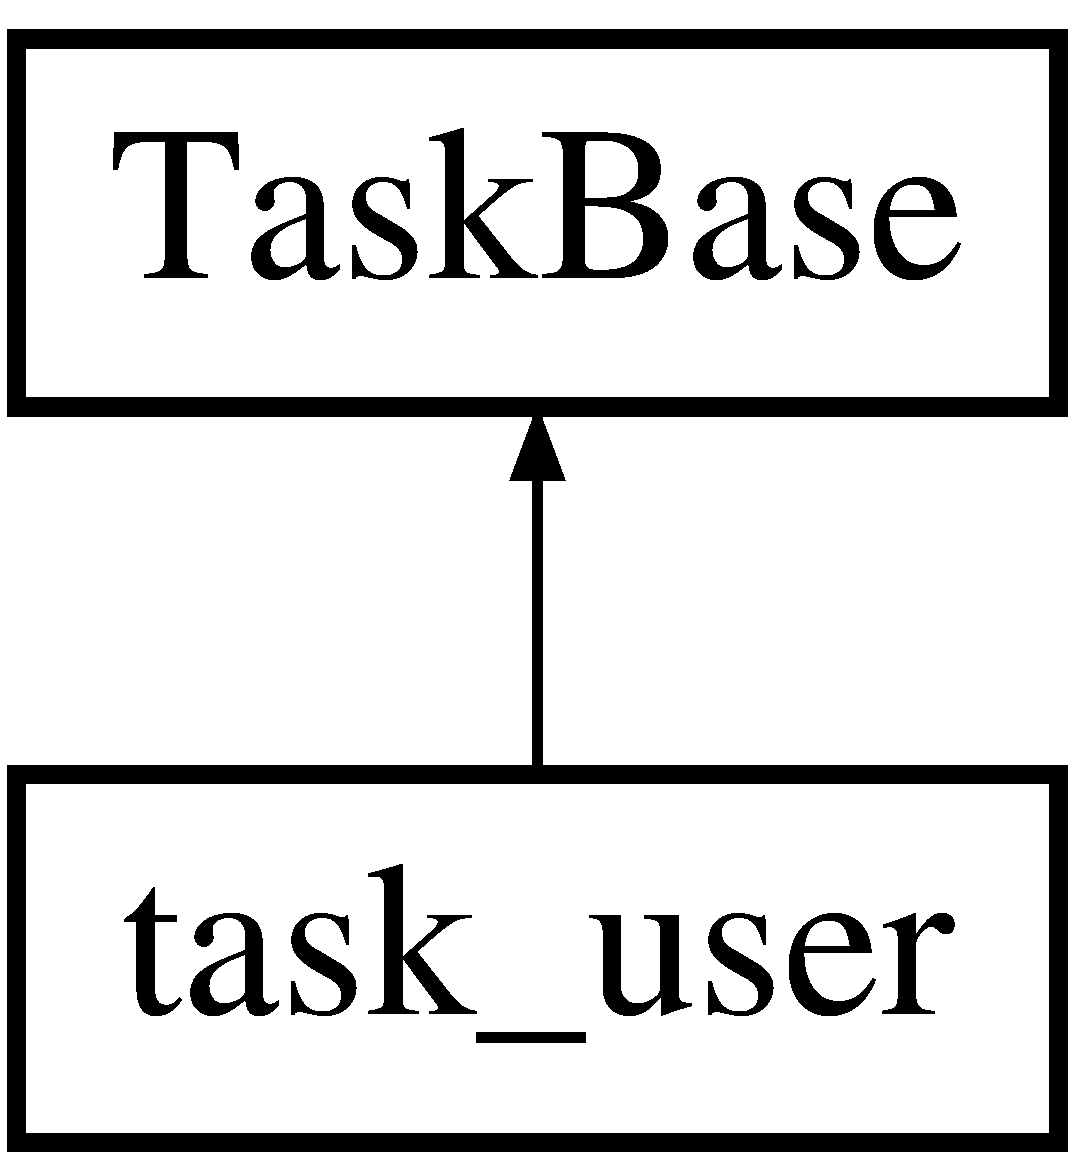
\includegraphics[height=2.000000cm]{classtask__user}
\end{center}
\end{figure}
\subsection*{Public Member Functions}
\begin{DoxyCompactItemize}
\item 
\hyperlink{classtask__user_a3aba77563b375bb14838800608da48bc}{task\+\_\+user} (const char $\ast$, unsigned port\+B\+A\+S\+E\+\_\+\+T\+Y\+PE, size\+\_\+t, emstream $\ast$)
\item 
void \hyperlink{classtask__user_adca6429d57be25e8d411414fc8ad75af}{run} (void)
\end{DoxyCompactItemize}
\subsection*{Protected Member Functions}
\begin{DoxyCompactItemize}
\item 
void \hyperlink{classtask__user_a75475060f83bae1e44bcc8a5c34015c7}{print\+\_\+help\+\_\+message} (void)
\item 
void \hyperlink{classtask__user_a105bebbd9cb1031154c3dfc3662db4a0}{show\+\_\+status} (void)
\end{DoxyCompactItemize}


\subsection{Detailed Description}
This task interacts with the user for force him/her to do what he/she is told. What a rude task this is. Then again, computers tend to be that way; if they\textquotesingle{}re polite with you, they\textquotesingle{}re probably spying on you. 

\subsection{Constructor \& Destructor Documentation}
\index{task\+\_\+user@{task\+\_\+user}!task\+\_\+user@{task\+\_\+user}}
\index{task\+\_\+user@{task\+\_\+user}!task\+\_\+user@{task\+\_\+user}}
\subsubsection[{\texorpdfstring{task\+\_\+user(const char $\ast$, unsigned port\+B\+A\+S\+E\+\_\+\+T\+Y\+P\+E, size\+\_\+t, emstream $\ast$)}{task_user(const char *, unsigned portBASE_TYPE, size_t, emstream *)}}]{\setlength{\rightskip}{0pt plus 5cm}task\+\_\+user\+::task\+\_\+user (
\begin{DoxyParamCaption}
\item[{const char $\ast$}]{a\+\_\+name, }
\item[{unsigned port\+B\+A\+S\+E\+\_\+\+T\+Y\+PE}]{a\+\_\+priority, }
\item[{size\+\_\+t}]{a\+\_\+stack\+\_\+size, }
\item[{emstream $\ast$}]{p\+\_\+ser\+\_\+dev}
\end{DoxyParamCaption}
)}\hypertarget{classtask__user_a3aba77563b375bb14838800608da48bc}{}\label{classtask__user_a3aba77563b375bb14838800608da48bc}
This constructor creates a new data acquisition task. Its main job is to call the parent class\textquotesingle{}s constructor which does most of the work. 
\begin{DoxyParams}{Parameters}
{\em a\+\_\+name} & A character string which will be the name of this task \\
\hline
{\em a\+\_\+priority} & The priority at which this task will initially run (default\+: 0) \\
\hline
{\em a\+\_\+stack\+\_\+size} & The size of this task\textquotesingle{}s stack in bytes (default\+: config\+M\+I\+N\+I\+M\+A\+L\+\_\+\+S\+T\+A\+C\+K\+\_\+\+S\+I\+ZE) \\
\hline
{\em p\+\_\+ser\+\_\+dev} & Pointer to a serial device (port, radio, SD card, etc.) which can be used by this task to communicate (default\+: N\+U\+LL) \\
\hline
\end{DoxyParams}


\subsection{Member Function Documentation}
\index{task\+\_\+user@{task\+\_\+user}!print\+\_\+help\+\_\+message@{print\+\_\+help\+\_\+message}}
\index{print\+\_\+help\+\_\+message@{print\+\_\+help\+\_\+message}!task\+\_\+user@{task\+\_\+user}}
\subsubsection[{\texorpdfstring{print\+\_\+help\+\_\+message(void)}{print_help_message(void)}}]{\setlength{\rightskip}{0pt plus 5cm}void task\+\_\+user\+::print\+\_\+help\+\_\+message (
\begin{DoxyParamCaption}
\item[{void}]{}
\end{DoxyParamCaption}
)\hspace{0.3cm}{\ttfamily [protected]}}\hypertarget{classtask__user_a75475060f83bae1e44bcc8a5c34015c7}{}\label{classtask__user_a75475060f83bae1e44bcc8a5c34015c7}
This method prints a simple help message. \index{task\+\_\+user@{task\+\_\+user}!run@{run}}
\index{run@{run}!task\+\_\+user@{task\+\_\+user}}
\subsubsection[{\texorpdfstring{run(void)}{run(void)}}]{\setlength{\rightskip}{0pt plus 5cm}void task\+\_\+user\+::run (
\begin{DoxyParamCaption}
\item[{void}]{}
\end{DoxyParamCaption}
)}\hypertarget{classtask__user_adca6429d57be25e8d411414fc8ad75af}{}\label{classtask__user_adca6429d57be25e8d411414fc8ad75af}
This method is called by the R\+T\+OS once to run the task loop for ever and ever.

This task interacts with the user for force him/her to do what he/she is told. It is just following the modern government model of \char`\"{}\+This is the land of the free...
free to do exactly what you\textquotesingle{}re told.\char`\"{} \index{task\+\_\+user@{task\+\_\+user}!show\+\_\+status@{show\+\_\+status}}
\index{show\+\_\+status@{show\+\_\+status}!task\+\_\+user@{task\+\_\+user}}
\subsubsection[{\texorpdfstring{show\+\_\+status(void)}{show_status(void)}}]{\setlength{\rightskip}{0pt plus 5cm}void task\+\_\+user\+::show\+\_\+status (
\begin{DoxyParamCaption}
\item[{void}]{}
\end{DoxyParamCaption}
)\hspace{0.3cm}{\ttfamily [protected]}}\hypertarget{classtask__user_a105bebbd9cb1031154c3dfc3662db4a0}{}\label{classtask__user_a105bebbd9cb1031154c3dfc3662db4a0}
This method displays information about the status of the system, including the following\+: \begin{DoxyItemize}
\item The name and version of the program \item The name, status, priority, and free stack space of each task \item Processor cycles used by each task \item Amount of heap space free and setting of R\+T\+OS tick timer \end{DoxyItemize}


The documentation for this class was generated from the following files\+:\begin{DoxyCompactItemize}
\item 
\hyperlink{task__user_8h}{task\+\_\+user.\+h}\item 
\hyperlink{task__user_8cpp}{task\+\_\+user.\+cpp}\end{DoxyCompactItemize}

\chapter{File Documentation}
\hypertarget{adc_8cpp}{}\section{adc.\+cpp File Reference}
\label{adc_8cpp}\index{adc.\+cpp@{adc.\+cpp}}
{\ttfamily \#include $<$stdlib.\+h$>$}\\*
{\ttfamily \#include $<$avr/io.\+h$>$}\\*
{\ttfamily \#include \char`\"{}rs232int.\+h\char`\"{}}\\*
{\ttfamily \#include \char`\"{}adc.\+h\char`\"{}}\\*
\subsection*{Functions}
\begin{DoxyCompactItemize}
\item 
emstream \& \hyperlink{adc_8cpp_afb33ca9fe94765ee57079e7feb03f975}{operator$<$$<$} (emstream \&serpt, \hyperlink{classadc}{adc} \&a2d)
\begin{DoxyCompactList}\small\item\em This overloaded operator \char`\"{}prints the A/\+D converter.\char`\"{}. \end{DoxyCompactList}\end{DoxyCompactItemize}
\subsection*{Variables}
\begin{DoxyCompactItemize}
\item 
uint16\+\_\+t {\bfseries sampleavg} = 0\hypertarget{adc_8cpp_a31bb5e230c2905f80a3d120d7f5f339a}{}\label{adc_8cpp_a31bb5e230c2905f80a3d120d7f5f339a}

\item 
uint16\+\_\+tint {\bfseries time} = 0\hypertarget{adc_8cpp_a23797b70f7783cbc35de405e4799d6e3}{}\label{adc_8cpp_a23797b70f7783cbc35de405e4799d6e3}

\item 
uint16\+\_\+t {\bfseries A\+D\+C\+Read} = 1536\hypertarget{adc_8cpp_a56be14b248ab73a7ebf561a9964c1ea1}{}\label{adc_8cpp_a56be14b248ab73a7ebf561a9964c1ea1}

\end{DoxyCompactItemize}


\subsection{Detailed Description}
This file contains a very simple A/D converter driver. This driver should be

Revisions\+: \begin{DoxyItemize}
\item 01-\/15-\/2008 J\+RR Original (somewhat useful) file \item 10-\/11-\/2012 J\+RR Less original, more useful file with Free\+R\+T\+OS mutex added \item 10-\/12-\/2012 J\+RR There was a bug in the mutex code, and it has been fixed\end{DoxyItemize}
License\+: This file is copyright 2015 by JR Ridgely and released under the Lesser G\+NU Public License, version 2. It intended for educational use only, but its use is not limited thereto. 

\subsection{Function Documentation}
\index{adc.\+cpp@{adc.\+cpp}!operator$<$$<$@{operator$<$$<$}}
\index{operator$<$$<$@{operator$<$$<$}!adc.\+cpp@{adc.\+cpp}}
\subsubsection[{\texorpdfstring{operator$<$$<$(emstream \&serpt, adc \&a2d)}{operator<<(emstream &serpt, adc &a2d)}}]{\setlength{\rightskip}{0pt plus 5cm}emstream\& operator$<$$<$ (
\begin{DoxyParamCaption}
\item[{emstream \&}]{serpt, }
\item[{{\bf adc} \&}]{a2d}
\end{DoxyParamCaption}
)}\hypertarget{adc_8cpp_afb33ca9fe94765ee57079e7feb03f975}{}\label{adc_8cpp_afb33ca9fe94765ee57079e7feb03f975}


This overloaded operator \char`\"{}prints the A/\+D converter.\char`\"{}. 

The precise meaning of print is left to the user to interpret; it should be something useful. For example, one might print the values of the configuration registers or show current readings from all the A/D channels. 
\begin{DoxyParams}{Parameters}
{\em serpt} & Reference to a serial port to which the printout will be printed \\
\hline
{\em a2d} & Reference to the A/D driver which is being printed \\
\hline
\end{DoxyParams}
\begin{DoxyReturn}{Returns}
A reference to the same serial device on which we write information. This is used to string together things to write with {\ttfamily $<$$<$} operators 
\end{DoxyReturn}

\hypertarget{adc_8h}{}\section{adc.\+h File Reference}
\label{adc_8h}\index{adc.\+h@{adc.\+h}}
{\ttfamily \#include \char`\"{}emstream.\+h\char`\"{}}\\*
{\ttfamily \#include \char`\"{}Free\+R\+T\+O\+S.\+h\char`\"{}}\\*
{\ttfamily \#include \char`\"{}task.\+h\char`\"{}}\\*
{\ttfamily \#include \char`\"{}queue.\+h\char`\"{}}\\*
{\ttfamily \#include \char`\"{}semphr.\+h\char`\"{}}\\*
\subsection*{Classes}
\begin{DoxyCompactItemize}
\item 
class \hyperlink{classadc}{adc}
\begin{DoxyCompactList}\small\item\em This class runs the A/D converter on an A\+VR processor. \end{DoxyCompactList}\end{DoxyCompactItemize}
\subsection*{Functions}
\begin{DoxyCompactItemize}
\item 
emstream \& \hyperlink{adc_8h_a6e6d1e227b216fe2a1fee9b0ea52180d}{operator$<$$<$} (emstream \&, \hyperlink{classadc}{adc} \&)
\begin{DoxyCompactList}\small\item\em This overloaded operator \char`\"{}prints the A/\+D converter.\char`\"{}. \end{DoxyCompactList}\end{DoxyCompactItemize}


\subsection{Detailed Description}
This file contains a very simple A/D converter driver. The driver is hopefully thread safe in Free\+R\+T\+OS due to the use of a mutex to prevent its use by multiple tasks at the same time. There is no protection from priority inversion, however, except for the priority elevation in the mutex.

Revisions\+: \begin{DoxyItemize}
\item 01-\/15-\/2008 J\+RR Original (somewhat useful) file \item 10-\/11-\/2012 J\+RR Less original, more useful file with Free\+R\+T\+OS mutex added \item 10-\/12-\/2012 J\+RR There was a bug in the mutex code, and it has been fixed\end{DoxyItemize}
License\+: This file is copyright 2012 by JR Ridgely and released under the Lesser G\+NU Public License, version 2. It intended for educational use only, but its use is not limited thereto. 

\subsection{Function Documentation}
\index{adc.\+h@{adc.\+h}!operator$<$$<$@{operator$<$$<$}}
\index{operator$<$$<$@{operator$<$$<$}!adc.\+h@{adc.\+h}}
\subsubsection[{\texorpdfstring{operator$<$$<$(emstream \&, adc \&)}{operator<<(emstream &, adc &)}}]{\setlength{\rightskip}{0pt plus 5cm}emstream\& operator$<$$<$ (
\begin{DoxyParamCaption}
\item[{emstream \&}]{serpt, }
\item[{{\bf adc} \&}]{a2d}
\end{DoxyParamCaption}
)}\hypertarget{adc_8h_a6e6d1e227b216fe2a1fee9b0ea52180d}{}\label{adc_8h_a6e6d1e227b216fe2a1fee9b0ea52180d}


This overloaded operator \char`\"{}prints the A/\+D converter.\char`\"{}. 

The precise meaning of print is left to the user to interpret; it should be something useful. For example, one might print the values of the configuration registers or show current readings from all the A/D channels. 
\begin{DoxyParams}{Parameters}
{\em serpt} & Reference to a serial port to which the printout will be printed \\
\hline
{\em a2d} & Reference to the A/D driver which is being printed \\
\hline
\end{DoxyParams}
\begin{DoxyReturn}{Returns}
A reference to the same serial device on which we write information. This is used to string together things to write with {\ttfamily $<$$<$} operators 
\end{DoxyReturn}


Definition at line 143 of file adc.\+cpp.



References adc\+::read\+\_\+once().


\hypertarget{main_8cpp}{}\section{main.\+cpp File Reference}
\label{main_8cpp}\index{main.\+cpp@{main.\+cpp}}
{\ttfamily \#include $<$stdlib.\+h$>$}\\*
{\ttfamily \#include $<$avr/io.\+h$>$}\\*
{\ttfamily \#include $<$avr/wdt.\+h$>$}\\*
{\ttfamily \#include $<$string.\+h$>$}\\*
{\ttfamily \#include \char`\"{}Free\+R\+T\+O\+S.\+h\char`\"{}}\\*
{\ttfamily \#include \char`\"{}task.\+h\char`\"{}}\\*
{\ttfamily \#include \char`\"{}queue.\+h\char`\"{}}\\*
{\ttfamily \#include \char`\"{}croutine.\+h\char`\"{}}\\*
{\ttfamily \#include \char`\"{}rs232int.\+h\char`\"{}}\\*
{\ttfamily \#include \char`\"{}time\+\_\+stamp.\+h\char`\"{}}\\*
{\ttfamily \#include \char`\"{}taskbase.\+h\char`\"{}}\\*
{\ttfamily \#include \char`\"{}textqueue.\+h\char`\"{}}\\*
{\ttfamily \#include \char`\"{}taskqueue.\+h\char`\"{}}\\*
{\ttfamily \#include \char`\"{}taskshare.\+h\char`\"{}}\\*
{\ttfamily \#include \char`\"{}shares.\+h\char`\"{}}\\*
{\ttfamily \#include \char`\"{}task\+\_\+brightness.\+h\char`\"{}}\\*
{\ttfamily \#include \char`\"{}task\+\_\+user.\+h\char`\"{}}\\*
\subsection*{Functions}
\begin{DoxyCompactItemize}
\item 
int \hyperlink{main_8cpp_a840291bc02cba5474a4cb46a9b9566fe}{main} (void)
\end{DoxyCompactItemize}
\subsection*{Variables}
\begin{DoxyCompactItemize}
\item 
Text\+Queue $\ast$ \hyperlink{main_8cpp_acd99bf5d187d4809af2f460a5415e904}{p\+\_\+print\+\_\+ser\+\_\+queue}
\end{DoxyCompactItemize}


\subsection{Detailed Description}
This file contains the \hyperlink{main_8cpp_a840291bc02cba5474a4cb46a9b9566fe}{main()} code for a program which runs the M\+E405 board for M\+E405 lab 1. This program currently uses obfuscated code to use an A/D converter to convert an analog signal into an L\+ED brightness via pulse width modulation. {\bfseries This} {\bfseries comment} {\bfseries is} {\bfseries quite} {\bfseries messed} {\bfseries up} {\bfseries and} {\bfseries the} {\bfseries student} {\bfseries should} {\bfseries fix} {\bfseries it} {\bfseries so} {\bfseries that} {\bfseries it} {\bfseries accurately} {\bfseries reflects} {\bfseries the} {\bfseries function} {\bfseries of} {\bfseries the} {\bfseries program} {\bfseries which} {\bfseries is} {\bfseries handed} {\bfseries in} {\bfseries for} {\bfseries this} {\bfseries assignment}.

Revisions\+: \begin{DoxyItemize}
\item 09-\/30-\/2012 J\+RR Original file was a one-\/file demonstration with two tasks \item 10-\/05-\/2012 J\+RR Split into multiple files, one for each task plus a main one \item 10-\/30-\/2012 J\+RR A hopefully somewhat stable version with global queue pointers and the new operator used for most memory allocation \item 11-\/04-\/2012 J\+RR Free\+R\+T\+OS Swoop demo program changed to a sweet test suite \item 01-\/05-\/2012 J\+RR Program reconfigured as M\+E405 Lab 1 starting point \item 03-\/28-\/2014 J\+RR Pointers to shared variables and queues changed to references \item 01-\/04-\/2015 J\+RR Names of share \& queue classes changed; allocated with new now\end{DoxyItemize}
License\+: This file is copyright 2015 by JR Ridgely and released under the Lesser G\+NU Public License, version 2. It intended for educational use only, but its use is not limited thereto. 

\subsection{Function Documentation}
\index{main.\+cpp@{main.\+cpp}!main@{main}}
\index{main@{main}!main.\+cpp@{main.\+cpp}}
\subsubsection[{\texorpdfstring{main(void)}{main(void)}}]{\setlength{\rightskip}{0pt plus 5cm}int main (
\begin{DoxyParamCaption}
\item[{void}]{}
\end{DoxyParamCaption}
)}\hypertarget{main_8cpp_a840291bc02cba5474a4cb46a9b9566fe}{}\label{main_8cpp_a840291bc02cba5474a4cb46a9b9566fe}
The main function sets up the R\+T\+OS. Some test tasks are created. Then the scheduler is started up; the scheduler runs until power is turned off or there\textquotesingle{}s a reset. \begin{DoxyReturn}{Returns}
This is a real-\/time microcontroller program which doesn\textquotesingle{}t return. Ever. 
\end{DoxyReturn}


\subsection{Variable Documentation}
\index{main.\+cpp@{main.\+cpp}!p\+\_\+print\+\_\+ser\+\_\+queue@{p\+\_\+print\+\_\+ser\+\_\+queue}}
\index{p\+\_\+print\+\_\+ser\+\_\+queue@{p\+\_\+print\+\_\+ser\+\_\+queue}!main.\+cpp@{main.\+cpp}}
\subsubsection[{\texorpdfstring{p\+\_\+print\+\_\+ser\+\_\+queue}{p_print_ser_queue}}]{\setlength{\rightskip}{0pt plus 5cm}Text\+Queue$\ast$ p\+\_\+print\+\_\+ser\+\_\+queue}\hypertarget{main_8cpp_acd99bf5d187d4809af2f460a5415e904}{}\label{main_8cpp_acd99bf5d187d4809af2f460a5415e904}
This is a print queue, descended from {\ttfamily emstream} so that things can be printed into the queue using the \char`\"{}$<$$<$\char`\"{} operator and they\textquotesingle{}ll come out the other end as a stream of characters. It\textquotesingle{}s used by tasks that send things to the user interface task to be printed. 
\hypertarget{shares_8h}{}\section{shares.\+h File Reference}
\label{shares_8h}\index{shares.\+h@{shares.\+h}}
\subsection*{Variables}
\begin{DoxyCompactItemize}
\item 
Text\+Queue $\ast$ \hyperlink{shares_8h_acd99bf5d187d4809af2f460a5415e904}{p\+\_\+print\+\_\+ser\+\_\+queue}
\end{DoxyCompactItemize}


\subsection{Detailed Description}
This file contains extern declarations for queues and other inter-\/task data communication objects used in a M\+E405/507/\+Free\+R\+T\+OS project.

Revisions\+: \begin{DoxyItemize}
\item 09-\/30-\/2012 J\+RR Original file was a one-\/file demonstration with two tasks \item 10-\/05-\/2012 J\+RR Split into multiple files, one for each task plus a main one \item 10-\/29-\/2012 J\+RR Reorganized with global queue and shared data references \item 01-\/04-\/2014 J\+RR Re-\/reorganized, allocating shares with new now\end{DoxyItemize}
License\+: This file is copyright 2015 by JR Ridgely and released under the Lesser G\+NU Public License, version 2. It intended for educational use only, but its use is not limited thereto. 

\subsection{Variable Documentation}
\index{shares.\+h@{shares.\+h}!p\+\_\+print\+\_\+ser\+\_\+queue@{p\+\_\+print\+\_\+ser\+\_\+queue}}
\index{p\+\_\+print\+\_\+ser\+\_\+queue@{p\+\_\+print\+\_\+ser\+\_\+queue}!shares.\+h@{shares.\+h}}
\subsubsection[{\texorpdfstring{p\+\_\+print\+\_\+ser\+\_\+queue}{p_print_ser_queue}}]{\setlength{\rightskip}{0pt plus 5cm}Text\+Queue$\ast$ p\+\_\+print\+\_\+ser\+\_\+queue}\hypertarget{shares_8h_acd99bf5d187d4809af2f460a5415e904}{}\label{shares_8h_acd99bf5d187d4809af2f460a5415e904}
This is a print queue, descended from {\ttfamily emstream} so that things can be printed into the queue using the \char`\"{}$<$$<$\char`\"{} operator and they\textquotesingle{}ll come out the other end as a stream of characters. It\textquotesingle{}s used by tasks that send things to the user interface task to be printed. 

Definition at line 71 of file main.\+cpp.



Referenced by main(), and task\+\_\+user\+::run().


\hypertarget{task__brightness_8cpp}{}\section{task\+\_\+brightness.\+cpp File Reference}
\label{task__brightness_8cpp}\index{task\+\_\+brightness.\+cpp@{task\+\_\+brightness.\+cpp}}
{\ttfamily \#include \char`\"{}textqueue.\+h\char`\"{}}\\*
{\ttfamily \#include \char`\"{}task\+\_\+brightness.\+h\char`\"{}}\\*
{\ttfamily \#include \char`\"{}shares.\+h\char`\"{}}\\*


\subsection{Detailed Description}
This file contains the code for a task class which controls the brightness of an L\+ED using a voltage measured from the A/D as input. The fun part\+: the brightness that is being controlled can be on another A\+VR computer, with signals being sent and received via wireless transceivers.

Revisions\+: \begin{DoxyItemize}
\item 09-\/30-\/2012 J\+RR Original file was a one-\/file demonstration with two tasks \item 10-\/05-\/2012 J\+RR Split into multiple files, one for each task \item 10-\/25-\/2012 J\+RR Changed to a more fully C++ version with class task\+\_\+sender \item 10-\/27-\/2012 J\+RR Altered from data sending task into L\+ED blinking class \item 11-\/04-\/2012 J\+RR Altered again into the multi-\/task monstrosity \item 12-\/13-\/2012 J\+RR Yet again transmogrified; now it controls L\+ED brightness\end{DoxyItemize}
License\+: This file is copyright 2012 by JR Ridgely and released under the Lesser G\+NU Public License, version 2. It intended for educational use only, but its use is not limited thereto. 
\hypertarget{task__brightness_8h}{}\section{task\+\_\+brightness.\+h File Reference}
\label{task__brightness_8h}\index{task\+\_\+brightness.\+h@{task\+\_\+brightness.\+h}}
{\ttfamily \#include $<$stdlib.\+h$>$}\\*
{\ttfamily \#include $<$avr/io.\+h$>$}\\*
{\ttfamily \#include \char`\"{}Free\+R\+T\+O\+S.\+h\char`\"{}}\\*
{\ttfamily \#include \char`\"{}task.\+h\char`\"{}}\\*
{\ttfamily \#include \char`\"{}queue.\+h\char`\"{}}\\*
{\ttfamily \#include \char`\"{}taskbase.\+h\char`\"{}}\\*
{\ttfamily \#include \char`\"{}time\+\_\+stamp.\+h\char`\"{}}\\*
{\ttfamily \#include \char`\"{}taskqueue.\+h\char`\"{}}\\*
{\ttfamily \#include \char`\"{}taskshare.\+h\char`\"{}}\\*
{\ttfamily \#include \char`\"{}rs232int.\+h\char`\"{}}\\*
{\ttfamily \#include \char`\"{}adc.\+h\char`\"{}}\\*
\subsection*{Classes}
\begin{DoxyCompactItemize}
\item 
class \hyperlink{classtask__brightness}{task\+\_\+brightness}
\begin{DoxyCompactList}\small\item\em This task controls the brightness of an L\+ED using an analog input from the A/D converter. \end{DoxyCompactList}\end{DoxyCompactItemize}


\subsection{Detailed Description}
This file contains the header for a task class that controls the brightness of an L\+ED using a voltage measured from the A/D as input. The fun part\+: the brightness that is being controlled can be on another A\+VR computer, with signals being sent and received via wireless transceivers.

Revisions\+: \begin{DoxyItemize}
\item 09-\/30-\/2012 J\+RR Original file was a one-\/file demonstration with two tasks \item 10-\/05-\/2012 J\+RR Split into multiple files, one for each task \item 10-\/25-\/2012 J\+RR Changed to a more fully C++ version with class task\+\_\+sender \item 10-\/27-\/2012 J\+RR Altered from data sending task into L\+ED blinking class \item 11-\/04-\/2012 J\+RR Altered again into the multi-\/task monstrosity \item 12-\/13-\/2012 J\+RR Yet again transmogrified; now it controls L\+ED brightness\end{DoxyItemize}
License\+: This file is copyright 2012 by JR Ridgely and released under the Lesser G\+NU Public License, version 2. It intended for educational use only, but its use is not limited thereto. 
\hypertarget{task__user_8cpp}{}\section{task\+\_\+user.\+cpp File Reference}
\label{task__user_8cpp}\index{task\+\_\+user.\+cpp@{task\+\_\+user.\+cpp}}
{\ttfamily \#include $<$avr/io.\+h$>$}\\*
{\ttfamily \#include $<$avr/wdt.\+h$>$}\\*
{\ttfamily \#include \char`\"{}task\+\_\+user.\+h\char`\"{}}\\*
\subsection*{Variables}
\begin{DoxyCompactItemize}
\item 
const Tick\+Type\+\_\+t \hyperlink{task__user_8cpp_a608f2ff6213a79bd1f25a29544aeaba5}{ticks\+\_\+to\+\_\+delay} = ((config\+T\+I\+C\+K\+\_\+\+R\+A\+T\+E\+\_\+\+HZ / 1000) $\ast$ 5)
\end{DoxyCompactItemize}


\subsection{Detailed Description}
This file contains source code for a user interface task for a M\+E405/\+Free\+R\+T\+OS test suite.

Revisions\+: \begin{DoxyItemize}
\item 09-\/30-\/2012 J\+RR Original file was a one-\/file demonstration with two tasks \item 10-\/05-\/2012 J\+RR Split into multiple files, one for each task \item 10-\/25-\/2012 J\+RR Changed to a more fully C++ version with class \hyperlink{classtask__user}{task\+\_\+user} \item 11-\/04-\/2012 J\+RR Modified from the data acquisition example to the test suite \item 01-\/04-\/2014 J\+RR Changed base class names to Task\+Base, Task\+Share, etc.\end{DoxyItemize}
License\+: This file is copyright 2012 by JR Ridgely and released under the Lesser G\+NU Public License, version 2. It intended for educational use only, but its use is not limited thereto. 

\subsection{Variable Documentation}
\index{task\+\_\+user.\+cpp@{task\+\_\+user.\+cpp}!ticks\+\_\+to\+\_\+delay@{ticks\+\_\+to\+\_\+delay}}
\index{ticks\+\_\+to\+\_\+delay@{ticks\+\_\+to\+\_\+delay}!task\+\_\+user.\+cpp@{task\+\_\+user.\+cpp}}
\subsubsection[{\texorpdfstring{ticks\+\_\+to\+\_\+delay}{ticks_to_delay}}]{\setlength{\rightskip}{0pt plus 5cm}const Tick\+Type\+\_\+t ticks\+\_\+to\+\_\+delay = ((config\+T\+I\+C\+K\+\_\+\+R\+A\+T\+E\+\_\+\+HZ / 1000) $\ast$ 5)}\hypertarget{task__user_8cpp_a608f2ff6213a79bd1f25a29544aeaba5}{}\label{task__user_8cpp_a608f2ff6213a79bd1f25a29544aeaba5}
This constant sets how many R\+T\+OS ticks the task delays if the user\textquotesingle{}s not talking. The duration is calculated to be about 5 ms. 
\hypertarget{task__user_8h}{}\section{task\+\_\+user.\+h File Reference}
\label{task__user_8h}\index{task\+\_\+user.\+h@{task\+\_\+user.\+h}}
{\ttfamily \#include $<$stdlib.\+h$>$}\\*
{\ttfamily \#include \char`\"{}Free\+R\+T\+O\+S.\+h\char`\"{}}\\*
{\ttfamily \#include \char`\"{}task.\+h\char`\"{}}\\*
{\ttfamily \#include \char`\"{}queue.\+h\char`\"{}}\\*
{\ttfamily \#include \char`\"{}rs232int.\+h\char`\"{}}\\*
{\ttfamily \#include \char`\"{}adc.\+h\char`\"{}}\\*
{\ttfamily \#include \char`\"{}time\+\_\+stamp.\+h\char`\"{}}\\*
{\ttfamily \#include \char`\"{}taskbase.\+h\char`\"{}}\\*
{\ttfamily \#include \char`\"{}taskqueue.\+h\char`\"{}}\\*
{\ttfamily \#include \char`\"{}textqueue.\+h\char`\"{}}\\*
{\ttfamily \#include \char`\"{}taskshare.\+h\char`\"{}}\\*
{\ttfamily \#include \char`\"{}shares.\+h\char`\"{}}\\*
\subsection*{Classes}
\begin{DoxyCompactItemize}
\item 
class \hyperlink{classtask__user}{task\+\_\+user}
\end{DoxyCompactItemize}
\subsection*{Macros}
\begin{DoxyCompactItemize}
\item 
\#define \hyperlink{task__user_8h_a2f10abd650e471fae2d7e8c63d41206a}{P\+R\+O\+G\+R\+A\+M\+\_\+\+V\+E\+R\+S\+I\+ON}~P\+MS (\char`\"{}M\+E405 Lab 1 Unmodified Program V0.\+01 \char`\"{})\hypertarget{task__user_8h_a2f10abd650e471fae2d7e8c63d41206a}{}\label{task__user_8h_a2f10abd650e471fae2d7e8c63d41206a}

\begin{DoxyCompactList}\small\item\em This macro defines a string that identifies the name and version of this program. \end{DoxyCompactList}\end{DoxyCompactItemize}


\subsection{Detailed Description}
This file contains header stuff for a user interface task for a M\+E507/\+Free\+R\+T\+OS test suite.

Revisions\+: \begin{DoxyItemize}
\item 09-\/30-\/2012 J\+RR Original file was a one-\/file demonstration with two tasks \item 10-\/05-\/2012 J\+RR Split into multiple files, one for each task \item 10-\/25-\/2012 J\+RR Changed to a more fully C++ version with class \hyperlink{classtask__user}{task\+\_\+user} \item 11-\/04-\/2012 J\+RR Modified from the data acquisition example to the test suite \item 01-\/04-\/2014 J\+RR Changed base class names to Task\+Base, Task\+Share, etc.\end{DoxyItemize}
License\+: This file is copyright 2012 by JR Ridgely and released under the Lesser G\+NU Public License, version 2. It intended for educational use only, but its use is not limited thereto. 
%--- End generated contents ---

% Index
\backmatter
\newpage
\phantomsection
\clearemptydoublepage
\addcontentsline{toc}{chapter}{Index}
\printindex

\end{document}
